\documentclass[10pt,a4paper]{article}
\usepackage[utf8]{inputenc}
\usepackage[english]{babel}
\usepackage[T1]{fontenc}
\usepackage{amsmath}
\usepackage{amsfonts}
\usepackage{amssymb}
\usepackage{graphicx}
\usepackage{listings}
\author{Milan Tepic, Ivan Antunovic, Kareem Elzayat, Peter von Zameck Glyscinski}
\title{Assignment 2 Team 5}
\bibliographystyle{plain}

\begin{document}
\maketitle
\section*{Task 1}
\subsection*{a)}
\begin{figure}[h]
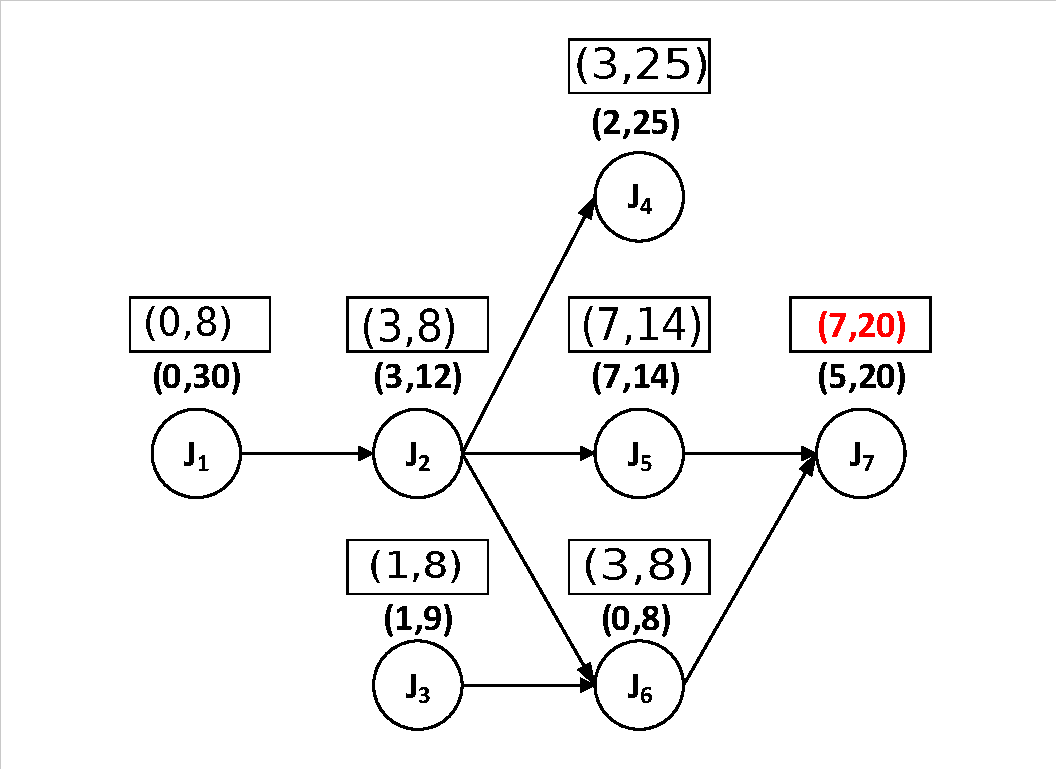
\includegraphics[width=\linewidth]{1a.pdf}
\caption{Effective Release time and Deadline.} 
\label{fig:1a}
\end{figure}
\newpage
\subsection*{b)}
\subsubsection*{i)}
The graph in figure \ref{fig:1bi} shows the network-flow graph with a feasible solution for the max-flow.
Edges are labeled with (flow|capacity).

\begin{figure}[h]
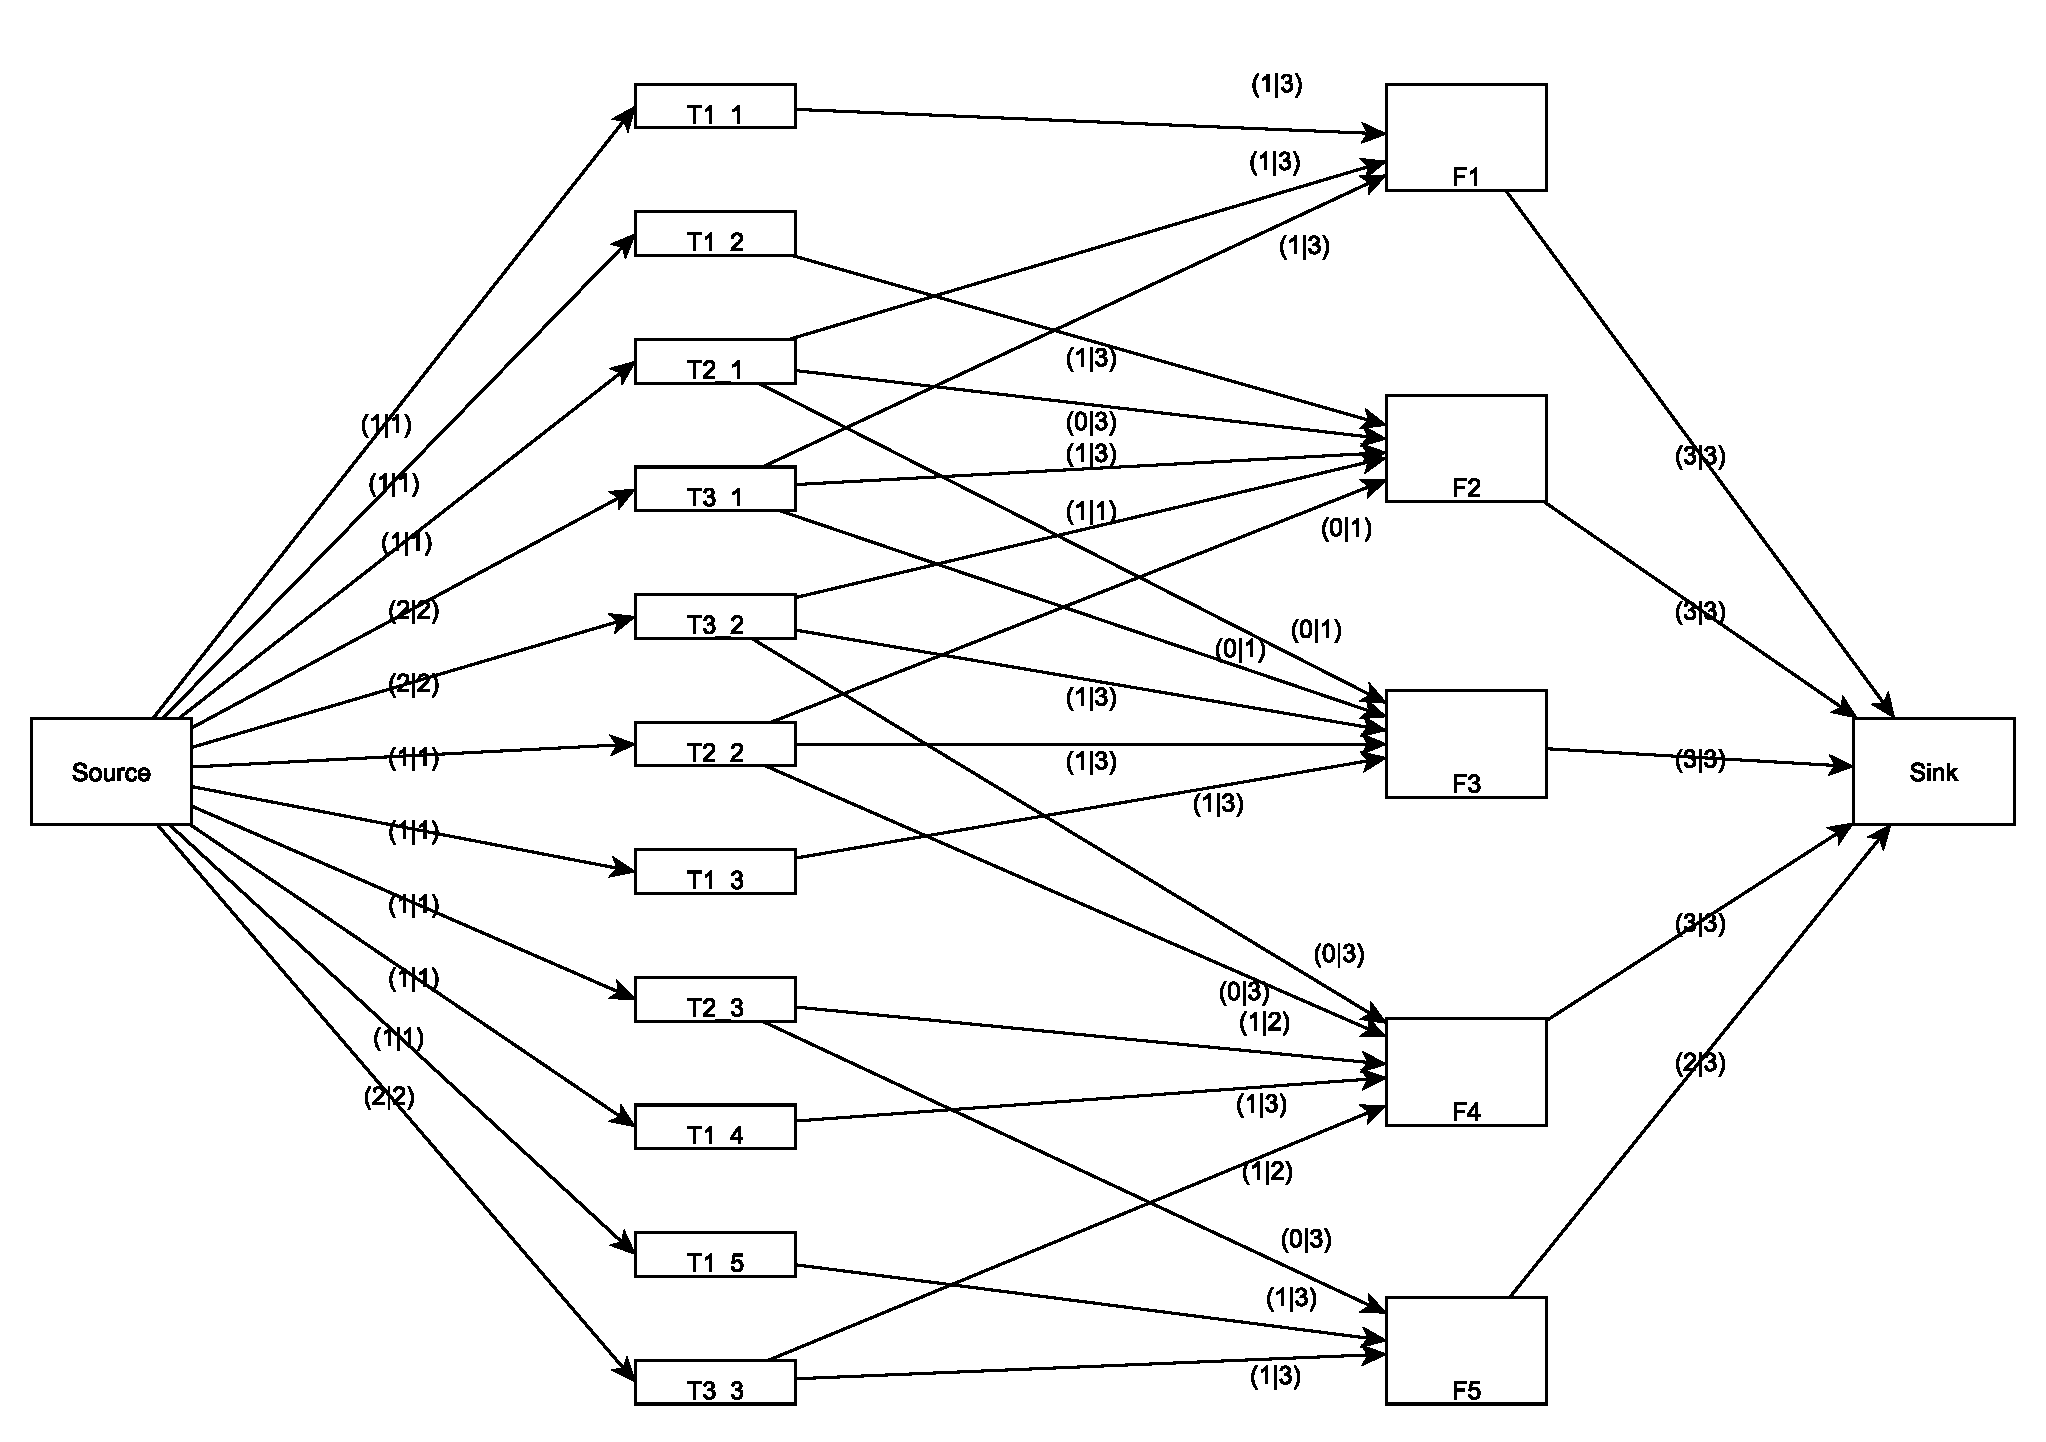
\includegraphics[width=\linewidth]{maxflow_1b.pdf}
\caption{Network flow graph for task 1 b) i).}
\label{fig:1bi}
\end{figure}

\begin{figure}[h]
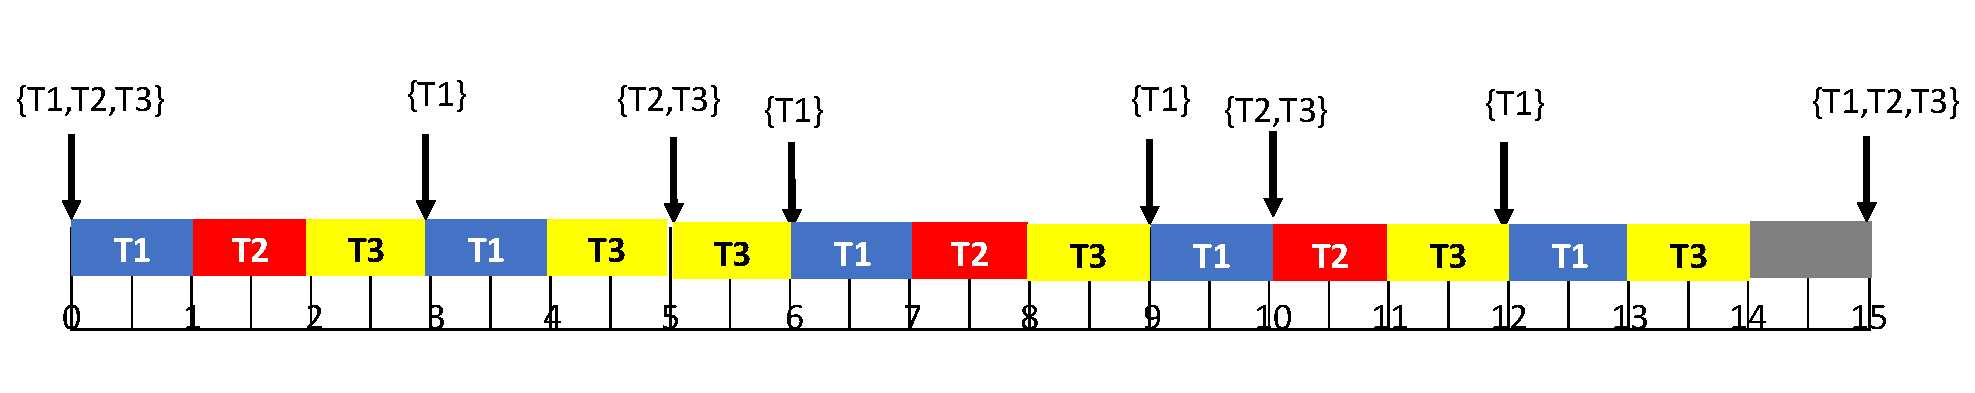
\includegraphics[width=\linewidth]{1b-timming-diagram.pdf}
\caption{Timming diagram for task 1 b) i).}
\label{fig:1biTimming}
\end{figure}

The resulting timming diagramm to the max-flow solution and also another proof that the task set is schedulable can be found in figure \ref{fig:1biTimming}.
\newpage
\section*{Task 2}
\subsection*{a)}

\begin{figure}[h]
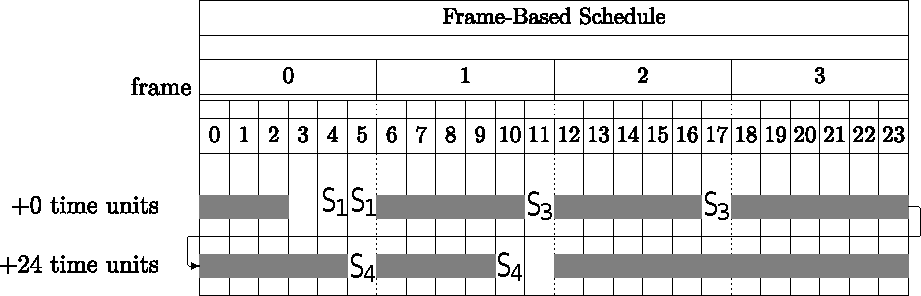
\includegraphics[width=\linewidth]{2a.pdf}
\label{fig:2a}
\end{figure}

\subsection*{b)}
$U = \frac{27}{42} = 0.642$
\newline
$U_A = \frac{2.5}{31} + \frac{3.375}{45} + \frac{2.25}{54} + \frac{2.5}{32} = 0.275$
\newline
$W_0 = \frac{8.25}{62} + \frac{12.625}{90} + \frac{6}{108} + \frac{8}{64} = 0.45$
\newline
$\lambda = \frac{1}{31} + \frac{1}{45} + \frac{1}{54} + \frac{1}{32} = 0.104$
\newline
$T_{queing} = \frac{W_0}{(1-U)^2[1 - \frac{U_A}{1 - U}]} = \frac{0.45}{(1-0.642)^2[1 - \frac{0.275}{1 - 0.642}]} = 15.144$
\newline
$T_{average} = \frac{\frac{2.5}{31} + \frac{3.375}{45} + \frac{2.25}{54} + \frac{2.5}{32}}{\lambda(1 - U)} = \frac{0.275}{0.104(1 - 0.642)} = 7.398$
\newline
$W = T_{average} + T_{queing} = 7.398 + 15.144 = 22.542$
\section*{Task 3}
\subsection*{a)}
Check with Utilization bound test:
\newline
$U = \frac{4}{15} + \frac{4}{20} + \frac{4}{30} + \frac{4}{60} = 0.67 \leq U_{RM}(4) = 4(2^{\frac{1}{4}} - 1) = 0.756$

Therefore the task set $T_1$ can be scheduled using RMS.

\subsection*{b)}
Check with Utilization bound test:
\newline
$U = \frac{4}{15} + \frac{4}{20} + \frac{8}{30} + \frac{8}{60} = 0.867 \nleq U_{RM}(4) = 4(2^{\frac{1}{4}} - 1) = 0.756$
Doesn't satisfy  utilization bound test.

Check with worst case simulation:
\newline
For task $A$: $4 \leq 15$
\newline
For task $B$: $C_B = (2 * 4) + 4 = 12 \leq 20$
\newline
For task $C$: $C_c = (2 * 4) + (2 * 4) + 8 = 24 \leq 30$
\newline
For task $D$: $C_d = (2 * 8) + (3 * 4) + (4 * 4) + 8 = 52 \leq 60$

Therefore the task set $T_2$ can be scheduled using RMS.

\subsection*{c)}
Since $D$ has the highest plriority we want to choose $x$ such that task $D$ gets a smaller deadline. 
For that we chose $x=4$ and get new task $D^\prime = (\frac{8}{4}, 60 - \frac{(4 - 1)60}{4}) = (2, 15)$
With this new task we are able to schedule task set $T_2$ with applied period transformation shown in figure \ref{fig:3c}.


\begin{figure}[!h]
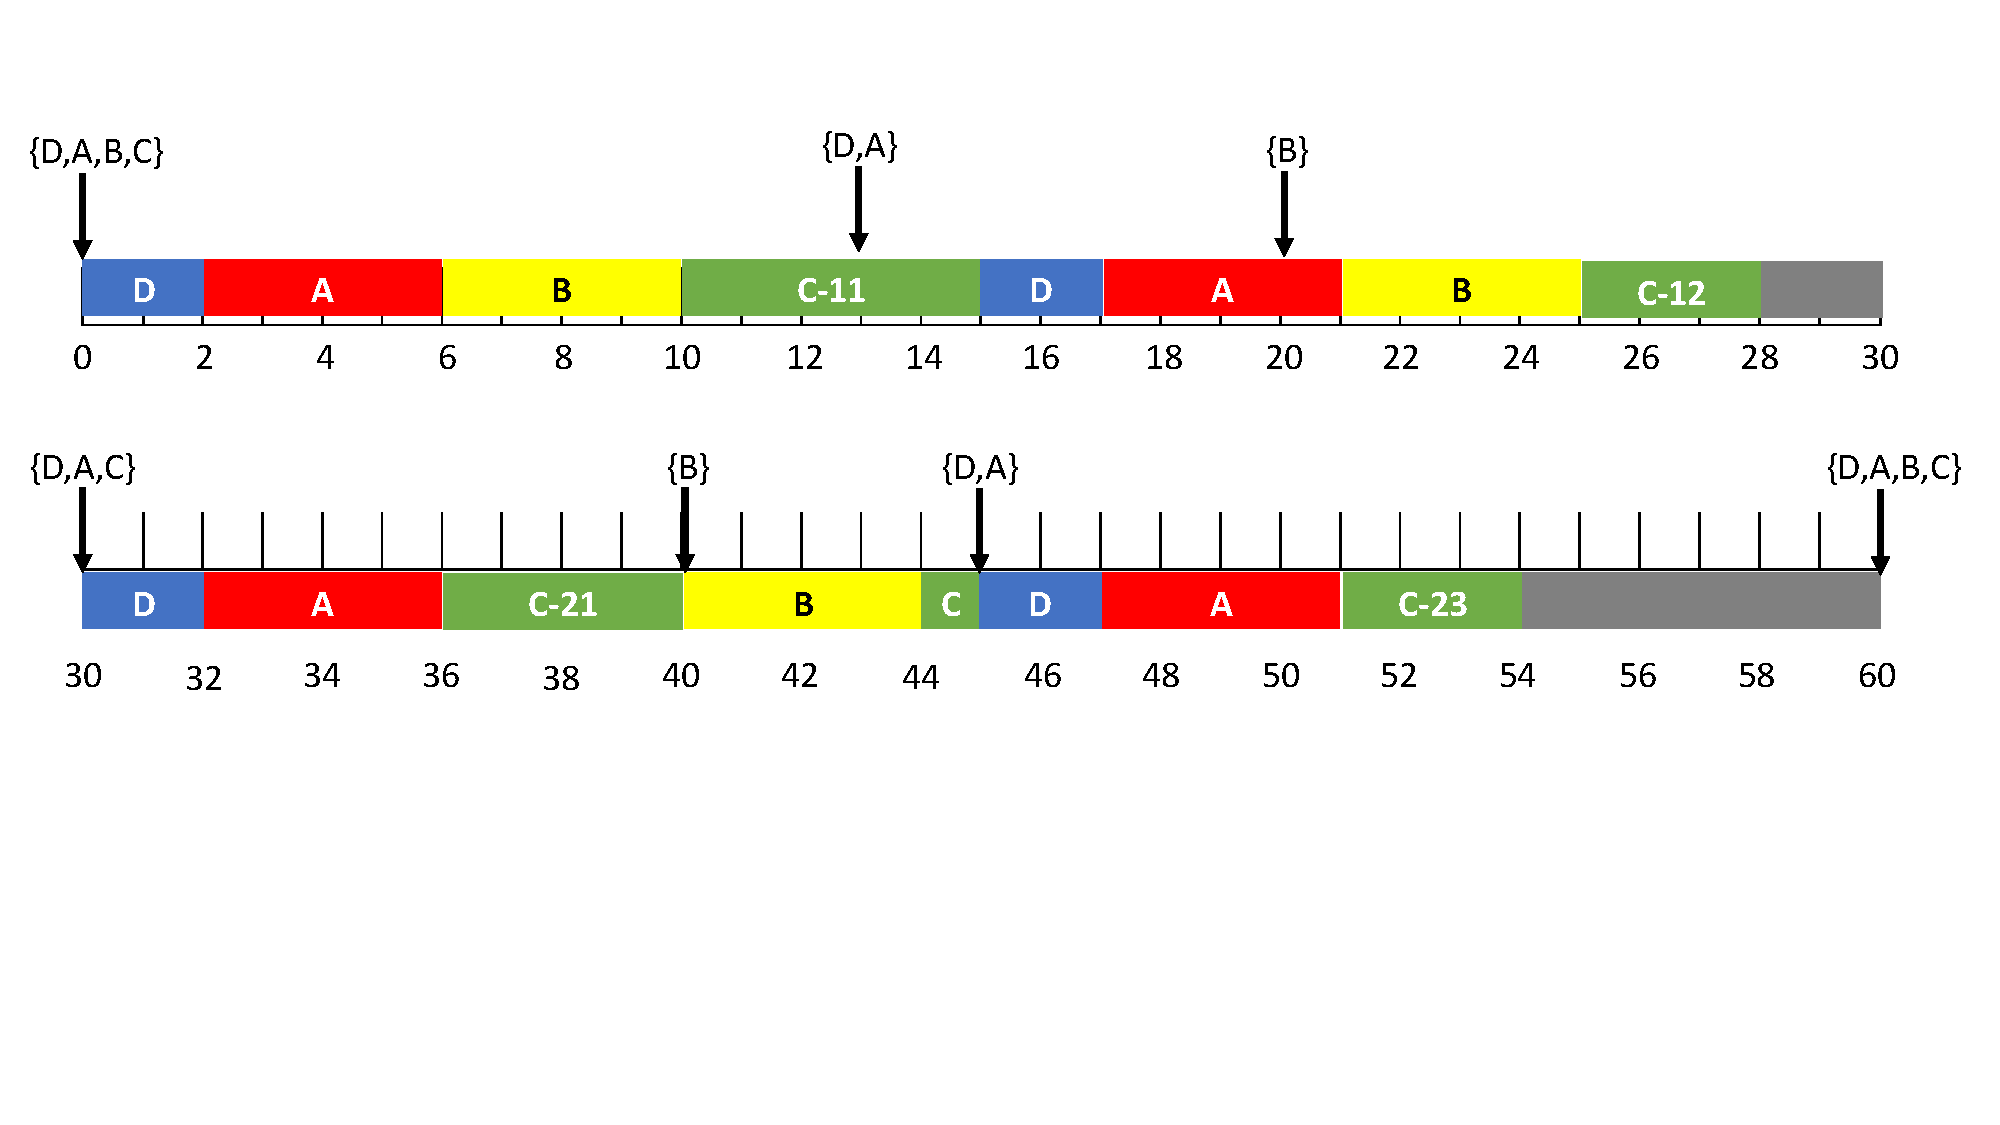
\includegraphics[width=\linewidth]{3c.pdf}
\caption{Timming diagram for task 3 c}
\label{fig:3c}
\end{figure}

\subsection*{d)}
Check with the bound test with blocking(Theorem 16.4\cite{Fan:2015:RES:2800613}):

$\frac{4}{15} = \frac{4}{15} \leq 1$
\newline
$\frac{4}{15} + \frac{4}{20} = 0.75 \leq 2(2^{\frac{1}{2}} - 1) = 0.83 $
\newline
$\frac{4}{15} + \frac{4}{20} + \frac{8}{30} + \frac{4}{30} = 0.87 \nleq 3(2^{\frac{1}{3}} - 1) = 0.78$


\bibliography{bibl}
\end{document}